%! TEX root = **/report.tex
\section{Analyzing network models}

\subsection{Watts-Strotgatz model (WS)}

The value of $p$ controls the amount of randomness in the
WS graph. When $p$ is small (close to 0), most of the edges are unchanged,
and the graph has high clustering and long average path lengths.
As $p$ increases, more edges get ``rewired'',
and the graph becomes more random, with lower clustering and
shorter average path lengths.

\Cref{fig:ws_model} shows the clustering coefficient and the average
shortest path length of the Watts-Strogatz model as a function of the
rewiring probability $p$. We used $n=1000$ nodes and $k=4$ edges per
node. In order to reduce the noise, we averaged the results over 10
different graphs for each configuration.

\begin{figure}[H]
    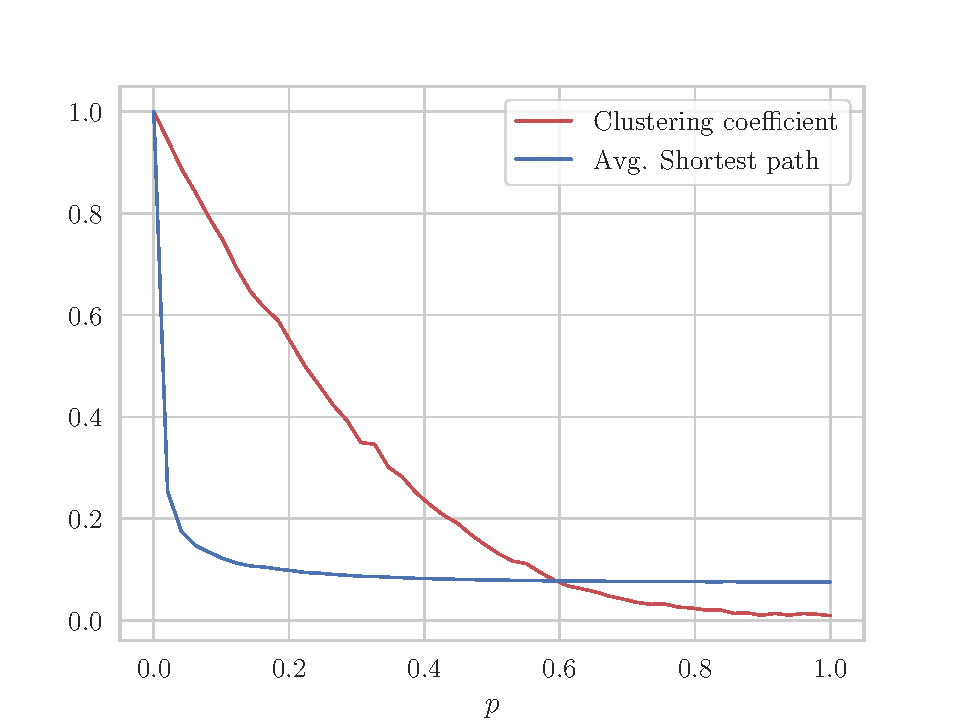
\includegraphics{figures/ws_model}
    \caption{Watts-Strotgatz model (WS) results}%
    \label{fig:ws_model}%
\end{figure}

We can observe a very steep drop in the average shortest path length
decreases much faster than the clustering coefficient. This is because
initially, the graph is a ring, therefore the average shortest path length is
quite big. However, with greater rewiring, there are more ``shortcuts'' to
reach any other node bypassing the initial ring structure, therefore, the shortest
path decreases very quickly. We can also see that the average shortest path stabilizes
and remains almost constant for $p>0.4$.

The decrease in the clustering coefficient is much slower, since the
much more edges need to be rewired in order to disconnect the nodes from
its neighbors.


\subsection{Barabasi-Albert model}

In a \emph{Barabasi-Albert} (BA) network, the degree distribution follows a power law,
which means that the probability of a node having a certain degree
 (i.e., the number of edges it is connected to) is inversely proportional
 to the degree raised to some power (typically denoted by $\gamma$).

The BA model is a generative model for growing networks that starts with
a small number of nodes and gradually adds new nodes over time.
Each new node is connected to $m$ existing nodes with a probability proportional to the degree of
the existing nodes. This process results in a \emph{scale-free} network,
where the degree distribution follows a power law of the form:
\begin{equation*}
    P(k) \propto k^{-\gamma}
\end{equation*}
where $P(k)$ is the probability of a node having degree $k$, and $\gamma$ is the power-law exponent.

The power-law exponent $\gamma$ for a BA network is typically around 2.1.
This means that the probability of a node having a high degree decreases rapidly with increasing
degree.
In other words, there are relatively few nodes with a high degree (i.e., many edges) compared to
the number of nodes with a low degree.

The power-law degree distribution of a BA network is a result of the preferential attachment mechanism,
which gives higher probability to nodes with a high degree
to attract new edges. This leads to the formation of a few highly connected nodes (hubs)
that dominate the network, and numerous low-degree nodes.

The \emph{Barabasi-Albert} (BA) model is a generative model for growing networks that is used
to study the structure and properties of real-world networks.

It is a simple model that captures some key features of many real-world networks,
such as the presence of highly connected nodes and the power-law degree distribution.

The BA model starts with a small number of nodes and
gradually adds new nodes over time. Each new node is connected to $m$ existing nodes with
a probability proportional to the degree of the existing nodes. This process results in a \emph{scale-free} network,
where the degree distribution follows a power law
(i.e., the probability of a node having a certain degree is inversely proportional to the degree raised to some power).

The degree distribution of most real-world networks follows a power-law distribution.

\begin{figure}[H]
    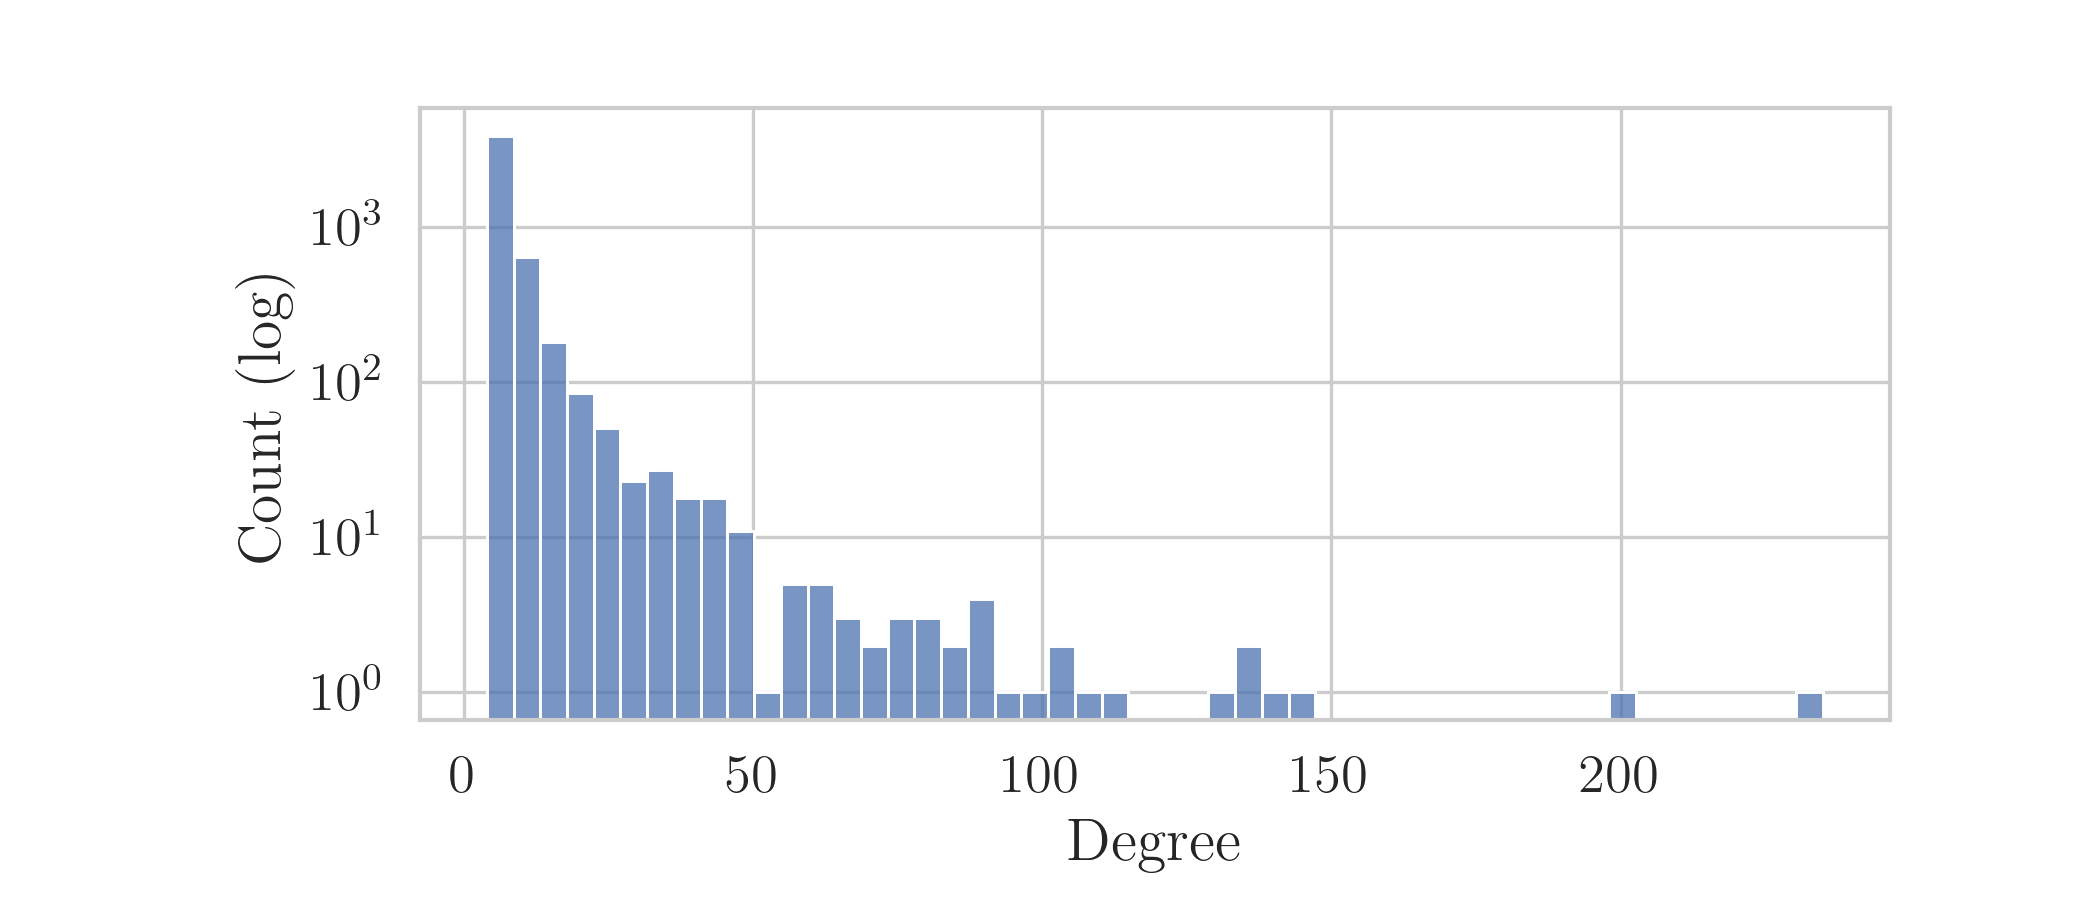
\includegraphics{figures/ba_dist_log.png}
    \caption{Barabasi-Albert model (BA) degree distribution histogram}%
    \label{fig:ba_degree_dist}%
\end{figure}

We built a BA network with $n=5000$ nodes and $m=4$, and then computed the degree distribution,
which we show in \cref{fig:ba_degree_dist}. Using this data, we can use \texttt{scipy.optimize.curve\_fit}
to fit it to the power law function $f(k) = a k^{-\gamma}$, and obtain the power-law exponent $\gamma$.
We do not need to convert frequency to a probability, since we only care about $\gamma$ and not
the $a$ constant. The result is $\gamma=2.514$, as shown in \cref{fig:ba_fit}.

\begin{figure}[H]
    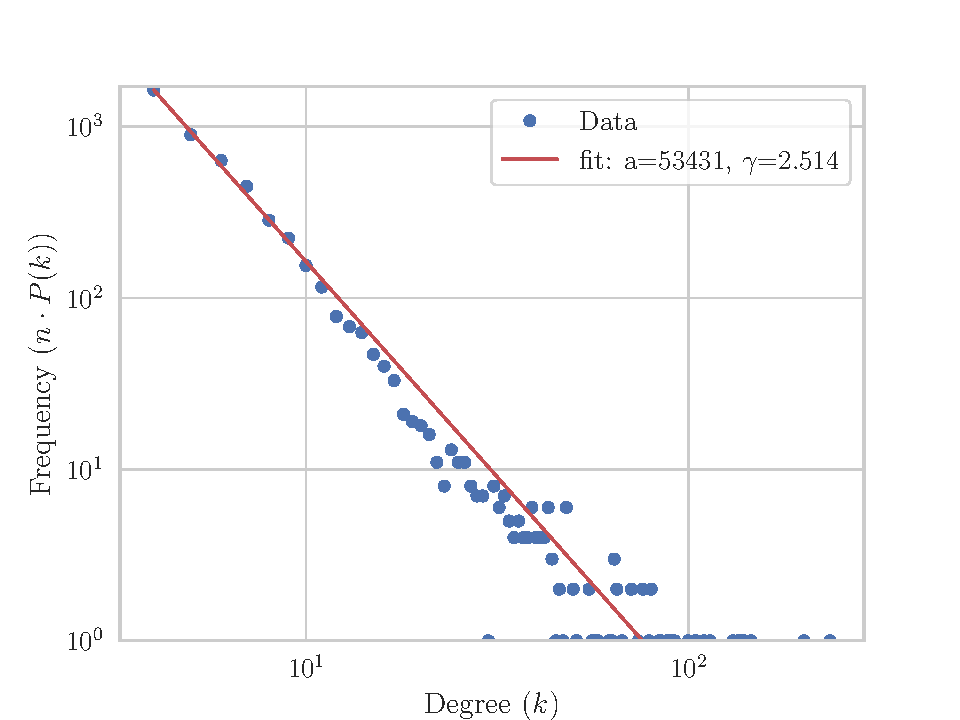
\includegraphics{figures/ba_fit}
    \caption{Barabasi-Albert model (BA) fit}%
    \label{fig:ba_fit}%
\end{figure}
